
%% bare_conf.tex
%% V1.3
%% 2007/01/11
%% by Michael Shell
%% See:
%% http://www.michaelshell.org/
%% for current contact information.
%%
%% This is a skeleton file demonstrating the use of IEEEtran.cls
%% (requires IEEEtran.cls version 1.7 or later) with an IEEE conference paper.
%%
%% Support sites:
%% http://www.michaelshell.org/tex/ieeetran/
%% http://www.ctan.org/tex-archive/macros/latex/contrib/IEEEtran/
%% and
%% http://www.ieee.org/

%%*************************************************************************
%% Legal Notice:
%% This code is offered as-is without any warranty either expressed or
%% implied; without even the implied warranty of MERCHANTABILITY or
%% FITNESS FOR A PARTICULAR PURPOSE! 
%% User assumes all risk.
%% In no event shall IEEE or any contributor to this code be liable for
%% any damages or losses, including, but not limited to, incidental,
%% consequential, or any other damages, resulting from the use or misuse
%% of any information contained here.
%%
%% All comments are the opinions of their respective authors and are not
%% necessarily endorsed by the IEEE.
%%
%% This work is distributed under the LaTeX Project Public License (LPPL)
%% ( http://www.latex-project.org/ ) version 1.3, and may be freely used,
%% distributed and modified. A copy of the LPPL, version 1.3, is included
%% in the base LaTeX documentation of all distributions of LaTeX released
%% 2003/12/01 or later.
%% Retain all contribution notices and credits.
%% ** Modified files should be clearly indicated as such, including  **
%% ** renaming them and changing author support contact information. **
%%
%% File list of work: IEEEtran.cls, IEEEtran_HOWTO.pdf, bare_adv.tex,
%%                    bare_conf.tex, bare_jrnl.tex, bare_jrnl_compsoc.tex
%%*************************************************************************

% *** Authors should verify (and, if needed, correct) their LaTeX system  ***
% *** with the testflow diagnostic prior to trusting their LaTeX platform ***
% *** with production work. IEEE's font choices can trigger bugs that do  ***
% *** not appear when using other class files.                            ***
% The testflow support page is at:
% http://www.michaelshell.org/tex/testflow/



% Note that the a4paper option is mainly intended so that authors in
% countries using A4 can easily print to A4 and see how their papers will
% look in print - the typesetting of the document will not typically be
% affected with changes in paper size (but the bottom and side margins will).
% Use the testflow package mentioned above to verify correct handling of
% both paper sizes by the user's LaTeX system.
%
% Also note that the "draftcls" or "draftclsnofoot", not "draft", option
% should be used if it is desired that the figures are to be displayed in
% draft mode.
%
\documentclass[conference]{IEEEtran}
\usepackage{blindtext, graphicx}

% correct bad hyphenation here
\hyphenation{op-tical net-works semi-conduc-tor}


\begin{document}
%
% paper title
% can use linebreaks \\ within to get better formatting as desired
\title{Review: Batik Classification using Transformation-Invariant Features}


% author names and affiliations
% use a multiple column layout for up to three different
% affiliations
\author{\IEEEauthorblockN{Yohanes Gultom}
\IEEEauthorblockA{Faculty of Computer Science\\
University of Indonesia\\
Depok, Indonesia\\
Email: yohanes.gultom@ui.ac.id}}

% make the title area
\maketitle


%\begin{abstract}
%%\boldmath
%Batik fabric is on of the most profound cultural heritage in Indonesia. Hence, continuous research on understanding it is necessary to preserve it. Despite of being one of the most common research task, Batik's pattern automatic classification still requires some improvement especially in regards to invariance dilemma. Convolutional neural network (ConvNet) is one od deep learning architecture which able to learn data representation in order to solve invariance dilemma in image classification. In this research, ConvNet is proposed as automatic classification architecture for Batik fabric natural images.
%\end{abstract}
%
%\begin{IEEEkeywords}
%Batik, convnet, deep learning, classification.
%\end{IEEEkeywords}

\section{Introduction}

Batik fabric is on of the most profound cultural heritage in Indonesia. Hence, continuous research on understanding it is necessary to preserve it. One of the most popular research topic is batik classification.

Since the most prominent feature of Batik is its uniquely recurring pattern (motifs), it's natural to consider it as a key to classification. To be more specific, recognition of Batik's motifs has been considered as one of the most successful technique in Batik classification \cite{azhar2015batik} \cite{nurhaida2015automatic} \cite{willy2013evaluation}. Classifications using other features such as color and contrast are showing potentials but need to be researched further \cite{moertini2005algorithms}.

In this paper, several researches about Batik motif-based classification are reviewed. They propose methods to extract transformation invariant features to improve classification accuracy on Batik images taken from various angles, distances and illumination levels. At the end of this paper, some possible works to extend the research in this topic further are also presented.

\section{Literature Review}

Recent researches in Batik classification can be divided into two groups: (1) Researches on classification using handcrafted features (eg. SIFT and SURF), and (2) researches on classification using automatically extracted features using deep learning.

\subsection{Classification using Handcrafted Features}

Since Batik classification has been researched for quite some time, current available methods are robust enough to noise addition, compression, and retouching of the input images. However most of them are still having difficulties with variance in transformations which involve either translation, rotation, scaling or combinations of them \cite{nurhaida2015automatic}. Recent improvements on Batik classification were motivated by the emergence of Scale-Invariant Feature Transform (SIFT)\cite{lowe2004distinctive} and Speeded up robust features (SURF)\cite{bay2006surf}. Both of these keypoint-based feature extraction methods are proposed to solve the transformation invariance dilemma.

SIFT keypoint is a circular image region with an orientation which can be obtained by detecting extrema of Difference of Gaussian (DoG) pyramid \cite{lowe2004distinctive}. It's defined by four parameters: center coordinates x and y, scale and its orientation (an angle expressed in radians) as shown in Figure \ref{fig_keypoint}. An image, for example Batik image, may contains multiple keypoints as shown in Figure \ref{fig_keypoint}. In order to be efficiently and effectively used as a feature for classification, the keypoint need to be represented as SIFT descriptor (Figure \ref{fig_sift_descriptor_1}). By definition it is a 3-dimensional spatial histogram of the image gradients characterizing a SIFT keypoint.

\begin{figure}[!t]
\centering
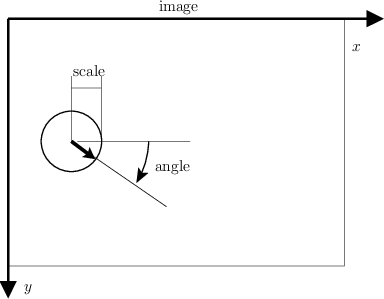
\includegraphics[width=2.0in]{sift-keypoint}
\caption{SIFT Keypoint}
\label{fig_keypoint}
\end{figure}

\begin{figure}[!t]
\centering
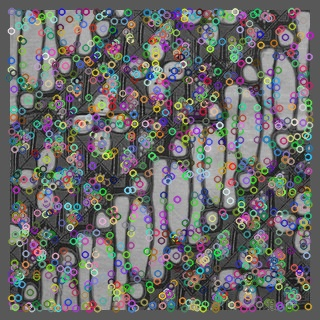
\includegraphics[width=2.0in]{batik-parang-keypoints}
\caption{SIFT keypoint}
\label{fig_batik_parang_keypoints}
\end{figure}

\begin{figure}[!t]
\centering
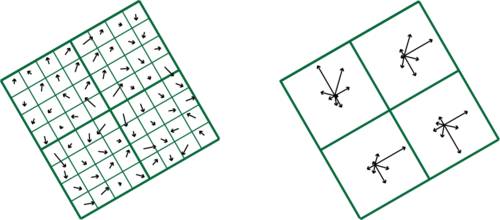
\includegraphics[width=2.0in]{sift-descriptor-1}
\caption{SIFT descriptor}
\label{fig_sift_descriptor_1}
\end{figure}

Recent research \cite{nurhaida2015automatic} proved that using SIFT descriptors to calculate similarity between Batik images can give 91.53\% accuracy. Voting Hough Transform was applied to the descriptors to eliminate mismatched keypoint candidates. This research suggested that the original SIFT descriptor matching shouldn't be directly used to calculate similarity of Batik images due to many numbers of mismatched keypoints. The method used in this research is described by diagram in Figure \ref{fig_sift_hough_voting_method}.

\begin{figure}[!t]
\centering
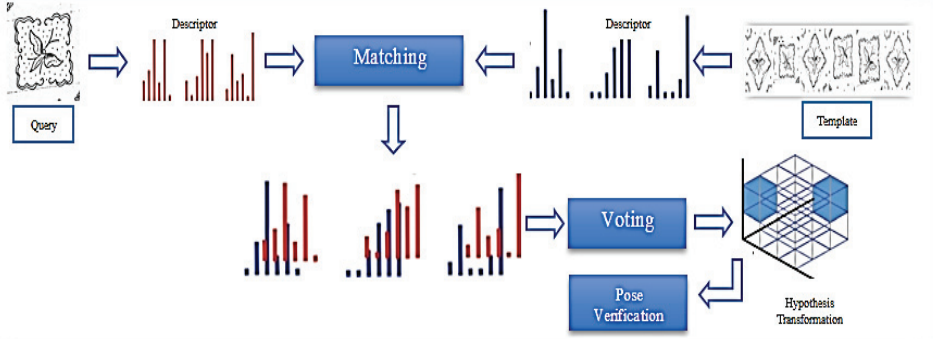
\includegraphics[width=3.0in]{sift-hough-voting-method}
\caption{SIFT with hough voting method for Batik classification}
\label{fig_sift_hough_voting_method}
\end{figure}

Another research \cite{azhar2015batik} proposed a classification method using support vector machine (SVM) fed by bag of words (BOF) features extracted using SIFT descriptors. In this research, SIFT descriptors also weren't used directly as features for SVM but were clustered using k-means vector quantization algorithm to build vocabularies. These visual vocabularies then used to describe each images and fed to SVM classifier. The experiment results showed very good average accuracy of 97.67\% for normal images, 95.47\% for rotated images and 79\% for scaled images. Besides that SIFT and bag of words made a good feature extractor, this research also concludes that further works need to handle scaled Batik image cases.

\begin{figure}[!t]
\centering
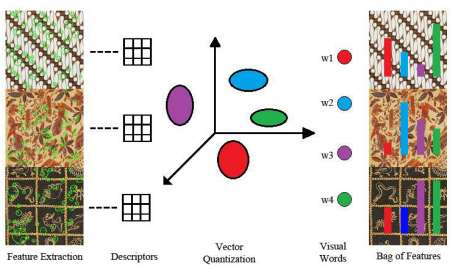
\includegraphics[width=3.0in]{sift-bag-of-words}
\caption{SIFT for building bag of words visual vocabularies}
\label{fig_sift_bag_of_words}
\end{figure}

An earlier research \cite{willy2013evaluation} proved that SURF can extract transformation invariant features faster than SIFT for classification of Songket, another Indonesian traditional fabric with motifs just like Batik. Unlike the others, this research used SIFT and SURF features directly to compute the matching scores between Songket images. The scores are calculated by (1) the number of matched keypoints and (2) the average total distance of the n-nearest keypoints. The result of experiments showed that the matching accuracy with SIFT features was 92-100\% and 65-97\% with SURF. With SURF features, the accuracy dropped quite significant if salt and pepper noises were added while SIFT was more stable. Apparently, this one wasn't paying much attention to transformation variance as it didn't apply transformation noise as in other research\cite{azhar2015batik}.

\begin{figure}[!t]
\centering
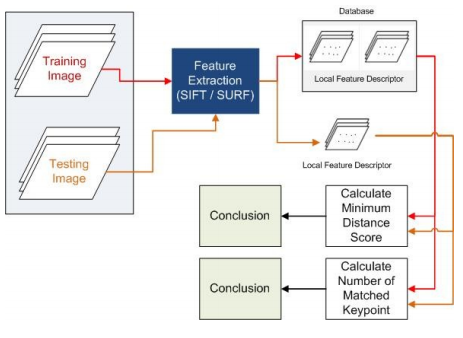
\includegraphics[width=3.0in]{songket-sift-vs-surf-methodology}
\caption{SIFT vs SURF method for Songket classification}
\label{fig_songket_sift_vs_surf_methodology}
\end{figure}

\subsection{Classification using Deep Learning}

Deep learning is a multilayer representation learning in artificial neural network \cite{lecun2015deep}. While representation learning itself is a method in machine learning to automatically extract/learn representation (features) from raw data. The representation of the raw data then can be used for recognition or classification task. Some fundamental deep learning architectures for instances are convolutional neural network (ConvNet), deep belief network (DBN), autoencoder (AE) and recurrent neural network (RNN). Despite of being an old idea, it was recently emerged due to the several factors: (1) discovery of new techniques (eg. pretraining \& dropout) and new activation functions (eg. ReLU), (2) enormous supply of data (big data), and (3) rapid improvement in computational hardware, especially GPU.

Although not yet many, the advent of deep learning also motivated a research on Batik classification using convolutional stacked autoencoder \cite{menzata2014sistem}. This research proposed the usage of convolutional transformations to reduce the input nodes of stacked autoencoder. The experiment showed that this deep architecture was able to achieve 81,73\% accuracy by using small patches of Batik for training. When noises were added its accuracy dropped to 49\% for gaussian noises, 61\% for rotations, 70\% for scalings and 75\% for illumination noises. Another research have shown that deep architecture such as convolutional neural network should be able to outperform handcrafted features such as SIFT\cite{fischer2014descriptor}. Therefore further research on Batik classification using deep learning architectures is encouraged.

% An example of a floating table. Note that, for IEEE style tables, the 
% \caption command should come BEFORE the table. Table text will default to
% \footnotesize as IEEE normally uses this smaller font for tables.
% The \label must come after \caption as always.
%
%\begin{table}[!t]
%% increase table row spacing, adjust to taste
%\renewcommand{\arraystretch}{1.3}
% if using array.sty, it might be a good idea to tweak the value of
% \extrarowheight as needed to properly center the text within the cells
%\caption{An Example of a Table}
%\label{table_example}
%\centering
%% Some packages, such as MDW tools, offer better commands for making tables
%% than the plain LaTeX2e tabular which is used here.
%\begin{tabular}{|c||c|}
%\hline
%One & Two\\
%\hline
%Three & Four\\
%\hline
%\end{tabular}
%\end{table}


\section{Future Works}

Due to the recent emergence of neural network \textit{deep learning}, many doors to improvement are opened for various field of research, especially image recognition and classification \cite{lecun2015deep}. The capability of deep neural networks to learn multilevel representation of image boosts the ability of machine to recognize patterns and objects in image invariant to transformations. Related research also has indicated that deep learning descriptor can outperform SIFT's \cite{fischer2014descriptor}. Therefore, using deep learning architecture on Batik classification may give better result that current approaches.

As suggested in the future works of related research, Batik classification should be attempted using architecture other than Convolutional Stacked Autoencoder such as Convulutional Neural Network (ConvNet)\cite{menzata2014sistem}. The same research also suggested to consider replacing SoftMax layer with other algorithm such as Naive Bayes Classifier (NBC) or Support Vector Machine (SVM).

Lastly, transferring learning model from another training session of similar deep architecture may provides better weight initialization \cite{simonyan2014very}. While we still need to train initialized network with Batik dataset, there is possibility that the classification result will be more accurate.

% Can use something like this to put references on a page
% by themselves when using endfloat and the captionsoff option.
\ifCLASSOPTIONcaptionsoff
  \newpage
\fi

\bibliography{proposal}
\bibliographystyle{IEEEtran}

% that's all folks
\end{document}


